\documentclass[]{article}
\usepackage{graphicx}
\usepackage{tikz,pgfplots}
\usepackage{xcolor}
\usetikzlibrary{positioning}

\begin{document}

%simple line
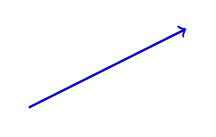
\begin{tikzpicture}
\draw[->,thick,blue](0,0)--(2,1);
\end{tikzpicture}
%circle and ellipse
\begin{tikzpicture}
\draw(0,0) circle(1);
\draw(2,0) circle(1.5in);
\draw(5,0) ellipse(10pt and 20pt);
\draw node at(3,0) {$f(x)$};
\filldraw(6,2) circle(0.1cm)node[anchor=west]{anchore node};
\end{tikzpicture}

\vspace{1in}
%rectangle without grid

\begin{tikzpicture}
%\draw(0,0) grid(5,4);
\draw[very thick,blue](0,0)rectangle(5,4);
\end{tikzpicture}


\begin{center}


\begin{tikzpicture}[transform canvas={scale=4.0}]
\draw[blue](0,1) arc(90:-90:0.5cm and 1cm);
\draw[dashed](0,1) arc(90:270:0.5cm and 1cm);
\draw(0,0)circle(1cm);
\filldraw[red](0,1)circle(0.05);
\filldraw[red](0,-1)circle(0.05);
\shade[ball color=blue!50!white,opacity=0.20](0,0)circle(0.05);
\end{tikzpicture}
\end{center}
\end{document}